\section{Deployment Module}

\subsection{Module Responsibility}
\noindent The Deployment module is responsible for transitioning trained machine learning models from the local training environment to production-ready serving environments. It packages model binaries and preprocessing pipelines, validates incoming API request schemas at runtime, tracks prediction telemetry, provides local and remote deployment targets (Docker, Heroku, AWS EC2), and maintains a lightweight model version control system (VCS).

The core files under \modulepath{accelera/src/deployment/} are:
\begin{itemize}[leftmargin=*]
  \item \modulepath{server.py}: The FastAPI web server exposing standard and batch inference endpoints.
  \item \modulepath{modelservice.py}: Manages model loading, preprocessor execution, and prediction routing.
  \item \modulepath{schema\_validation.py}: Performs runtime validation and data coercion using Great Expectations.
  \item \modulepath{tracking.py}: Records asynchronous prediction inputs, outputs, and latencies.
  \item \modulepath{deployment.py}: The orchestrator containing CLI commands for Local, Heroku, and EC2 deployments.
  \item \modulepath{vcs.py}: The model version control system managing staging, commits, and rollbacks.
\end{itemize}

\subsection{Modular Decomposition}

\subsubsection{Model Serving Subsystem}
\noindent Model serving is built on FastAPI and Uvicorn to handle concurrent HTTP requests. The subsystem loads the model and preprocessors via \texttt{ModelService}, which inspects the configuration (\texttt{config.json}) to locate the serialized artifacts. During execution, it runs input data through any fitted preprocessors in sequence before invoking the model's prediction method. A web-based graphical user interface (GUI) is dynamically rendered based on the expected input features, allowing users to submit single predictions interactively. Figure~\ref{fig:serving_architecture} shows the block diagram of the model serving architecture.

\begin{figure}[H]
\centering
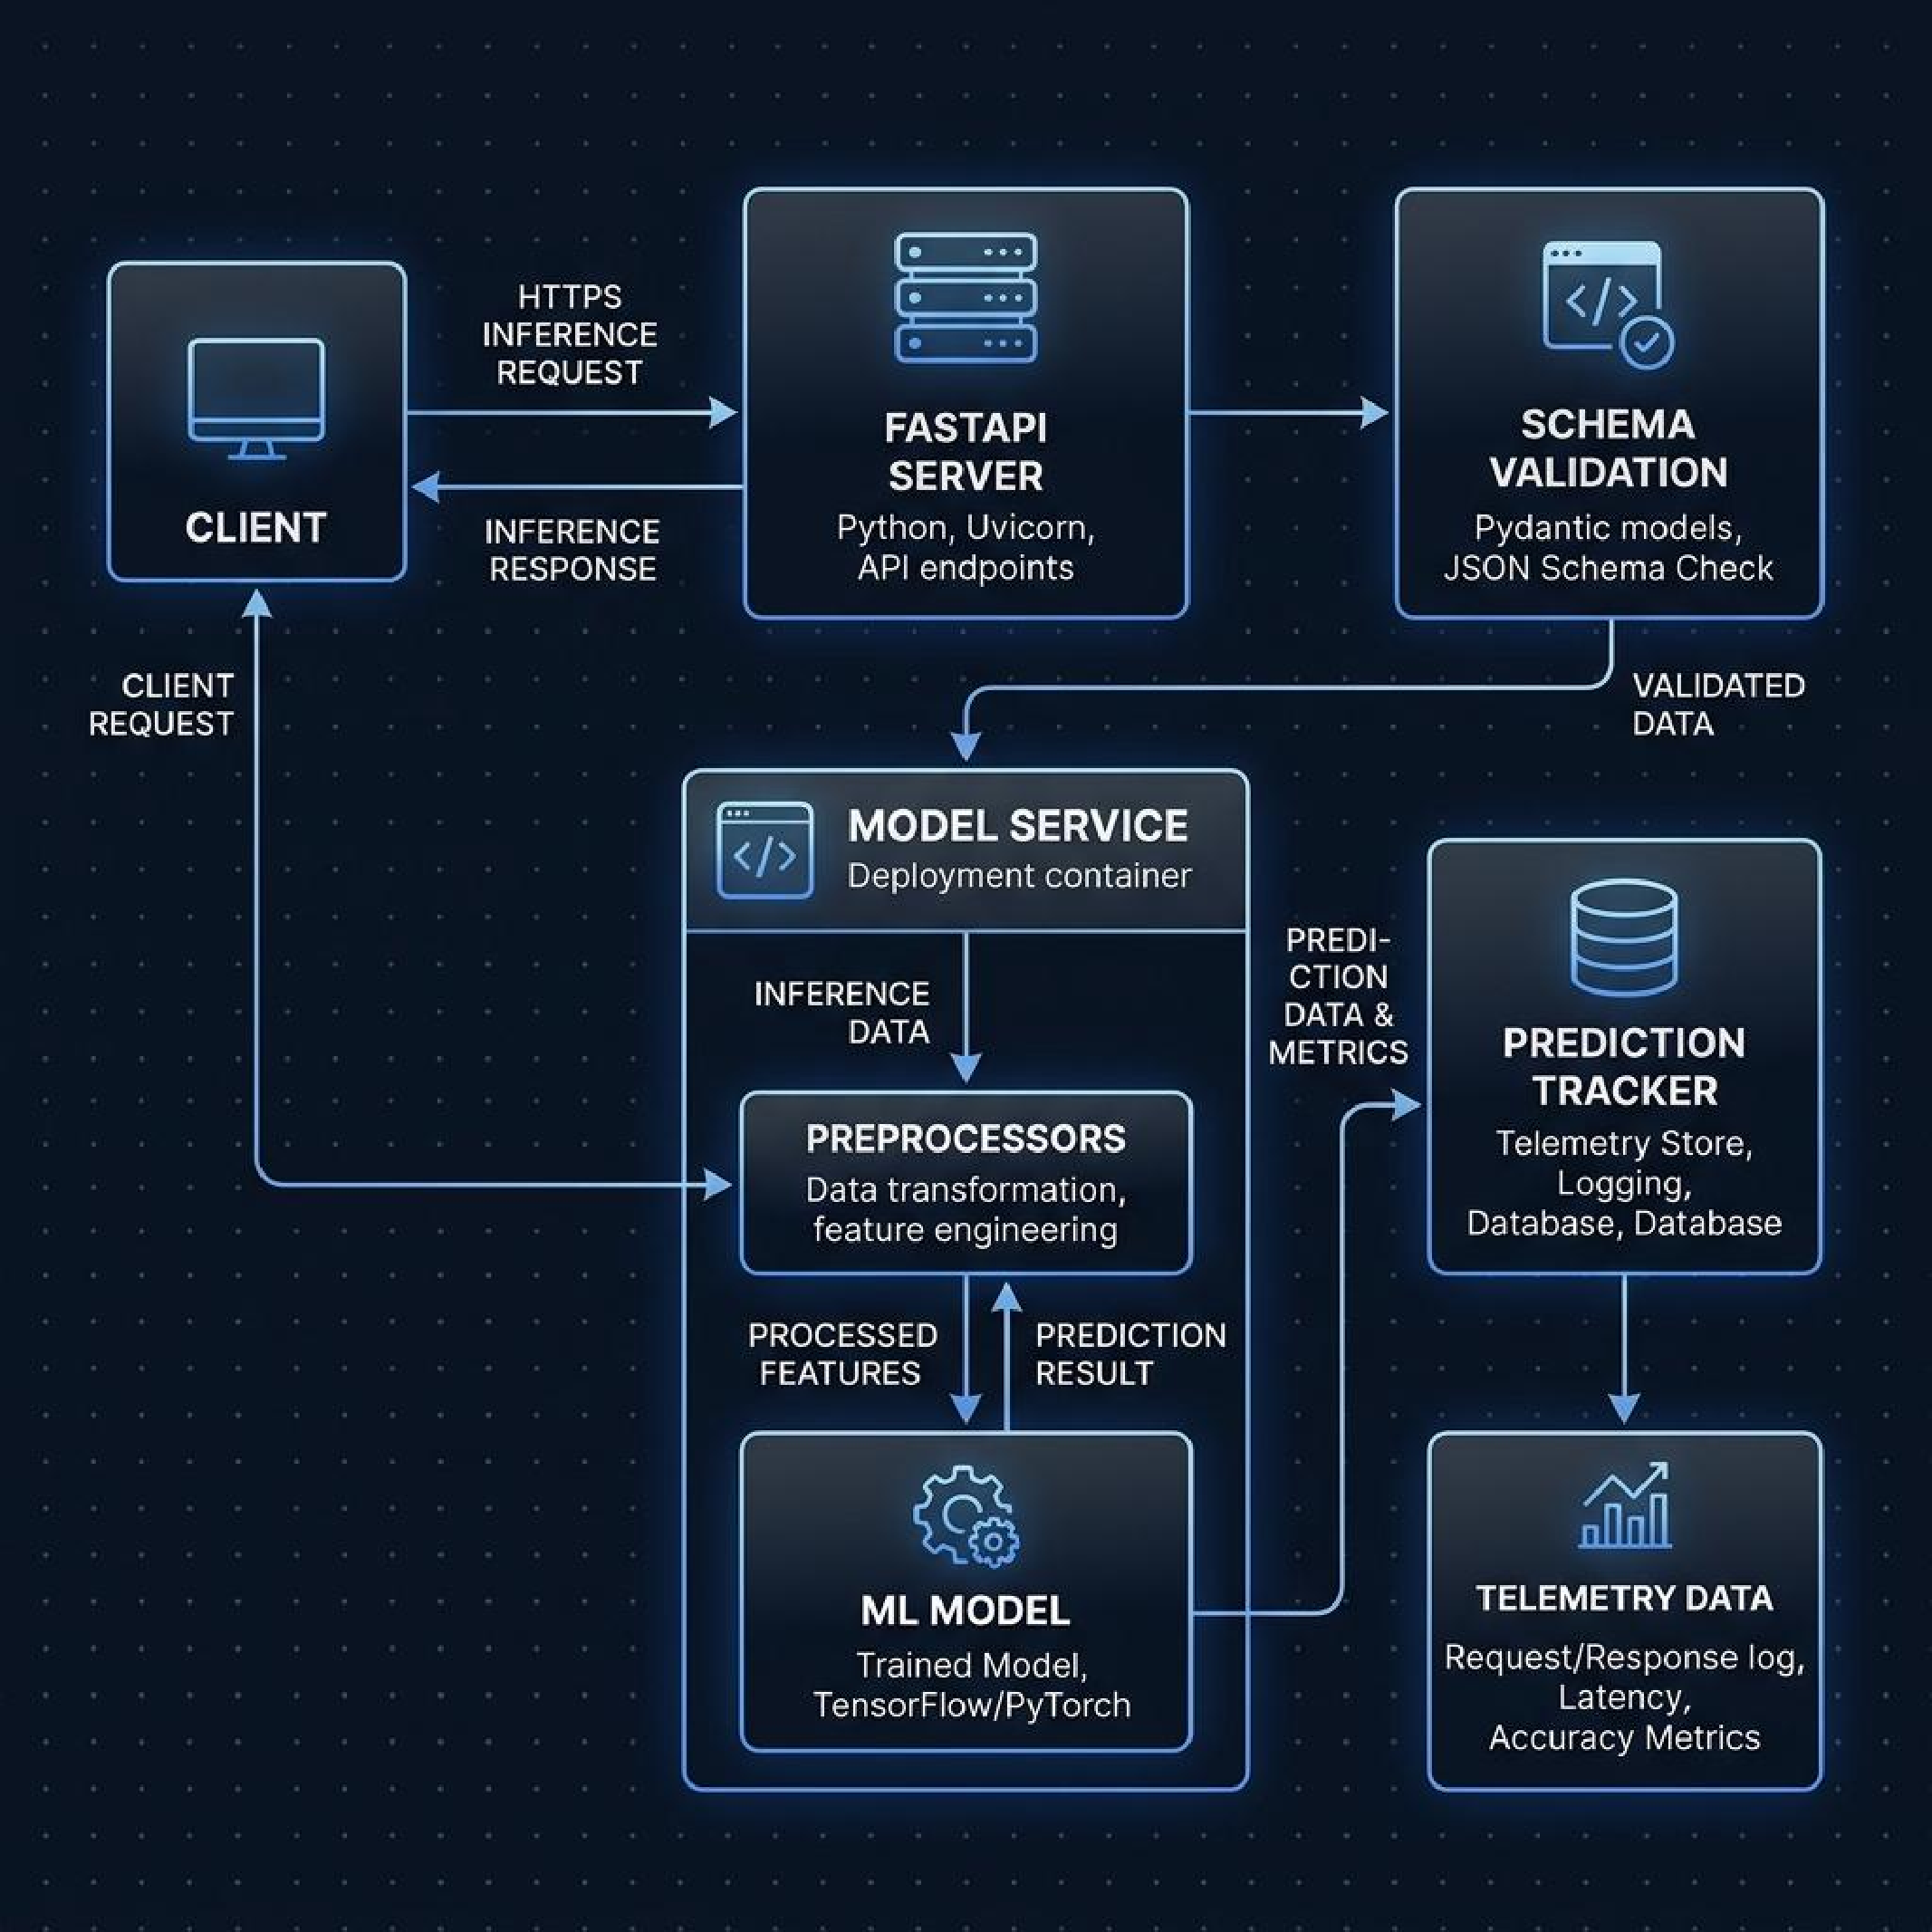
\includegraphics[width=0.85\textwidth]{imgs/serving_architecture.pdf}
\caption{Model Serving Architecture and Execution Flow}
\label{fig:serving_architecture}
\end{figure}

\noindent The following methods and files implement the serving logic:
\begin{itemize}[leftmargin=*]
  \item \modulepath{modelservice.py}:
    \begin{itemize}
      \item \texttt{ModelService.load()}: Parses \texttt{config.json} to discover active model configuration. It opens and loads the main estimator file (e.g. \texttt{model.pkl}) and any auxiliary preprocessors (e.g. scalers or encoders) from the models directory.
      \item \texttt{ModelService.predict(input\_data, validate=True)}: Performs prediction. If validation is active, it calls \texttt{validate\_input(input\_data)} to receive validated and coerced values, converts the inputs into a NumPy array, adjusts dimensions, applies all loaded preprocessor transforms sequentially, and calls the underlying estimator's \texttt{predict()} method.
    \end{itemize}
  \item \modulepath{server.py}:
    \begin{itemize}
      \item \texttt{\_predict(input\_data, endpoint, filename=None)}: Coordinates serving telemetry. It records starting timestamps using \texttt{time.perf\_counter()}, executes model prediction via \texttt{ModelService.predict()}, calculates API response latencies, and logs metrics to the telemetry storage.
      \item \texttt{/predict} and \texttt{/predict/csv} Endpoints: Standard HTTP POST methods. The first endpoint receives a structured JSON payload, while the second parses uploaded CSV files into Pandas DataFrames.
      \item \texttt{/gui} and \texttt{/health} Endpoints: The GUI endpoint returns the dynamic interactive testing form via \texttt{\_render\_gui(schema)}, while the health endpoint serves load balancers with standard status checks.
    \end{itemize}
\end{itemize}

\subsubsection{Runtime Schema Validation}
\noindent To prevent invalid inputs from causing model crashes or silent degradation, incoming payloads are validated against a schema specified in the configuration. The validation layer uses Great Expectations to construct an ephemeral data source context. Columns are validated for expected names, missing entries, unexpected inputs, and value bounds (e.g., minimum and maximum thresholds). Data types are coerced automatically (e.g., matching string, boolean, integer, or floating-point formats) to match the training format, raising a structured \texttt{SchemaValidationError} if coercion fails.

\noindent The schema validation system is implemented in \modulepath{schema\_validation.py}:
\begin{itemize}[leftmargin=*]
  \item \texttt{InputSchema.\_\_init\_\_(config)}: Extracts features and limits from configuration. If schema validation is enabled, it requests a Great Expectations context (\texttt{gx.get\_context()}), generates a unique UUID-based data source, registers a pandas-based DataFrame data asset, and configures a whole-dataframe batch definition.
  \item \texttt{InputSchema.validate(input\_data)}: Normalizes the input payload into a DataFrame. It checks for expected column presence, detects extra or missing features, runs the Great Expectations expectation suite, and executes type coercion.
  \item \texttt{InputSchema.coerce\_columns(df, errors)}: Loops through features to coerce types. It casts strings to numerical columns using \texttt{pd.to\_numeric(..., errors='coerce')}, checks for integer constraints (\texttt{value \% 1 == 0}), and processes boolean symbols (such as replacing \texttt{"true"}/\texttt{"false"} with python booleans).
  \item \texttt{InputSchema.to\_dataframe(input\_data)}: Utility method to convert list, dict, or DataFrame structures into standard Pandas format.
\end{itemize}

\subsubsection{Telemetry and Request Tracking}
\noindent Production deployments capture inference requests and runtime metrics using a lightweight tracking layer. When enabled, the tracker logs prediction inputs, model outputs, processing latencies (measured in milliseconds), and timestamps. To avoid performance degradation on the prediction path, logging is written incrementally to a JSON lines (\texttt{.jsonl}) file.

\noindent Telemetry tracking is implemented in \modulepath{tracking.py}:
\begin{itemize}[leftmargin=*]
  \item \texttt{PredictionTracker.\_\_init\_\_(config)}: Sets up the file system paths and creates/opens the telemetry log file.
  \item \texttt{PredictionTracker.log\_prediction(inputs, outputs, latency, status)}: Formats request parameters, response targets, server latency, and datetime strings into a single-line JSON string and appends it to the logging stream.
\end{itemize}

\subsubsection{Deployment Pipeline Orchestration}
\noindent The orchestration engine automates containerizing and launching the service across three distinct environments. It stages the codebase, copies project dependency requirements, and builds dockerized containers to ensure portability and reproducibility across platforms.
\begin{enumerate}[leftmargin=*]
  \item \textbf{Local Docker}: Generates a clean \texttt{Dockerfile} using a Python slim base image, stops any conflicting containers on the target port, builds the container image locally, and runs it.
  \item \textbf{Heroku}: Authenticates with the Heroku CLI and pushes/releases the Docker container using Heroku's Container Registry.
  \item \textbf{AWS EC2}: Creates an SSH transport connection and synchronizes the staging directory to the target host using \texttt{rsync} (excluding Python cache directories). It installs and starts the Docker daemon, builds the container on the instance, and executes local health check probes before verifying the public web endpoint.
\end{enumerate}

\begin{figure}[H]
\centering
\makebox[\textwidth][c]{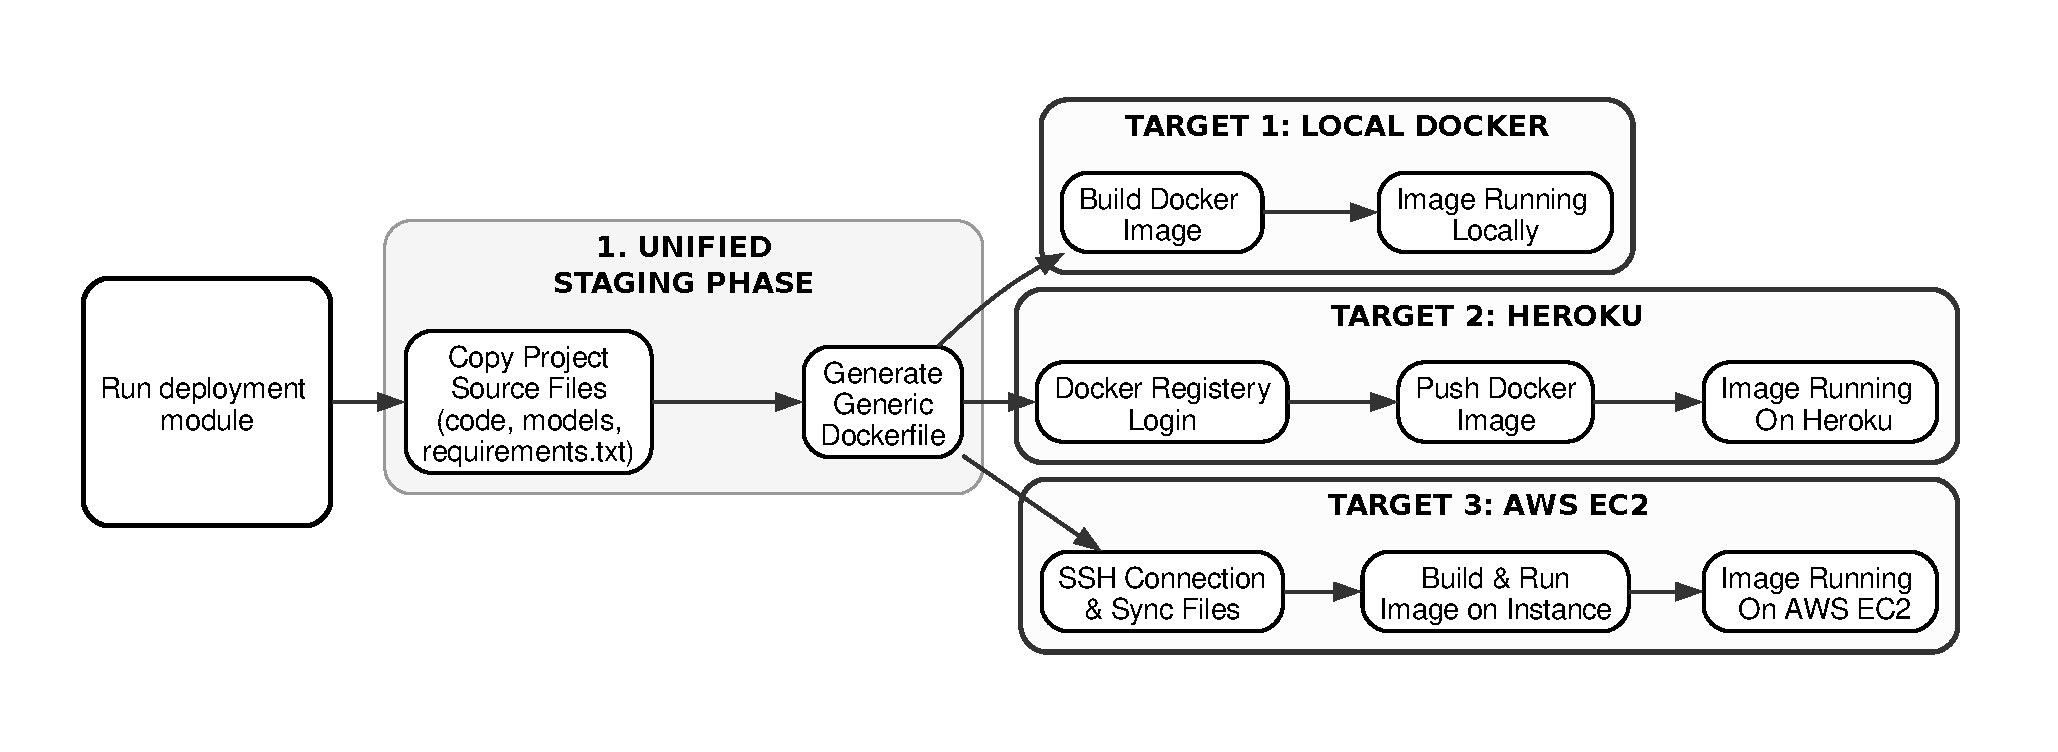
\includegraphics[width=1.2\textwidth]{dots/deployment_targets.pdf}}
\caption{Multi-Target Deployment Orchestration Flow}
\label{fig:orchestration_flow}
\end{figure}

\subsubsection{Model Version Control (VCS)}
\noindent The internal VCS provides reproducibility for deployed pipelines. It calculates a stable SHA-1 hash for each commit based on its timestamp and commit message. Models and configurations are archived into an \texttt{experiments/} subdirectory. The system maintains a global index (\texttt{experiments.json}) containing parent-child commit histories, HEAD references, and active deployed markers, facilitating rollbacks and deployments of historical model versions.

\noindent The version control subsystem is implemented in \modulepath{vcs.py}:
\begin{itemize}[leftmargin=*]
  \item \texttt{calculate\_hash(timestamp, message)}: Computes the 7-character SHA-1 hash value that acts as the commit identifier.
  \item \texttt{init(args)}: Configures the repository workspace by creating directories and saving the default index (\texttt{experiments.json}).
  \texttt{commit(args)}: Validates that models exist, generates a commit hash, copies the active configuration and models to \texttt{experiments/<hash>/}, and appends the commit entry to the registry.
  \item \texttt{log(args)}: Lists all recorded commits, showing details such as commit hash, creation date, message, and deploy status.
  \item \texttt{show(args)}: Displays the details and settings of a target commit.
  \item \texttt{deploy(args)}: Deploys a specific commit by copying its stored model files and configuration back into the active runtime workspace.
\end{itemize}

\begin{figure}[H]
\centering
\makebox[\textwidth][c]{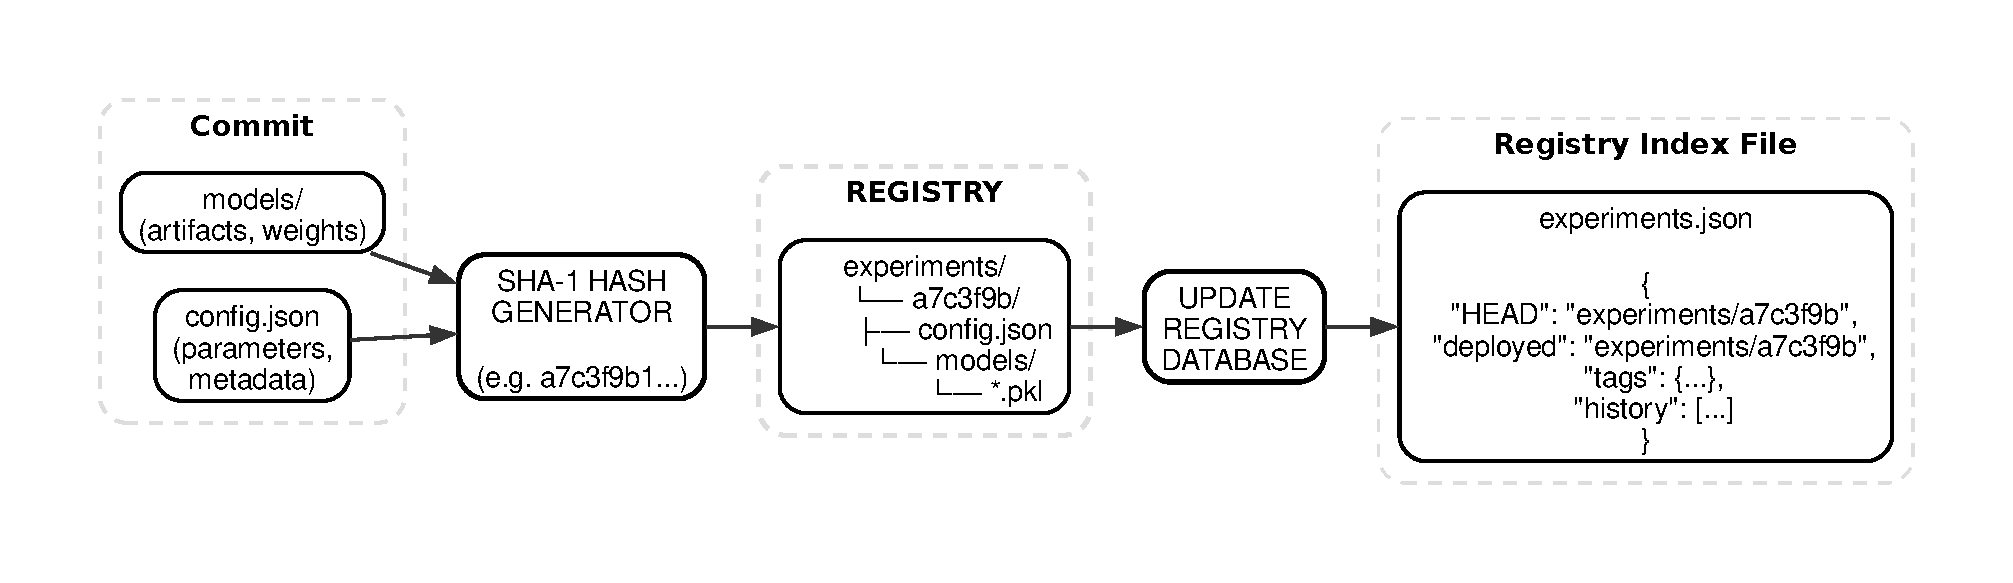
\includegraphics[width=1.2\textwidth]{dots/deployment_commit.pdf}}
\caption{VCS Commit Workflow}
\label{fig:vcs_commit_flow}
\end{figure}

\begin{figure}[H]
\centering
\makebox[\textwidth][c]{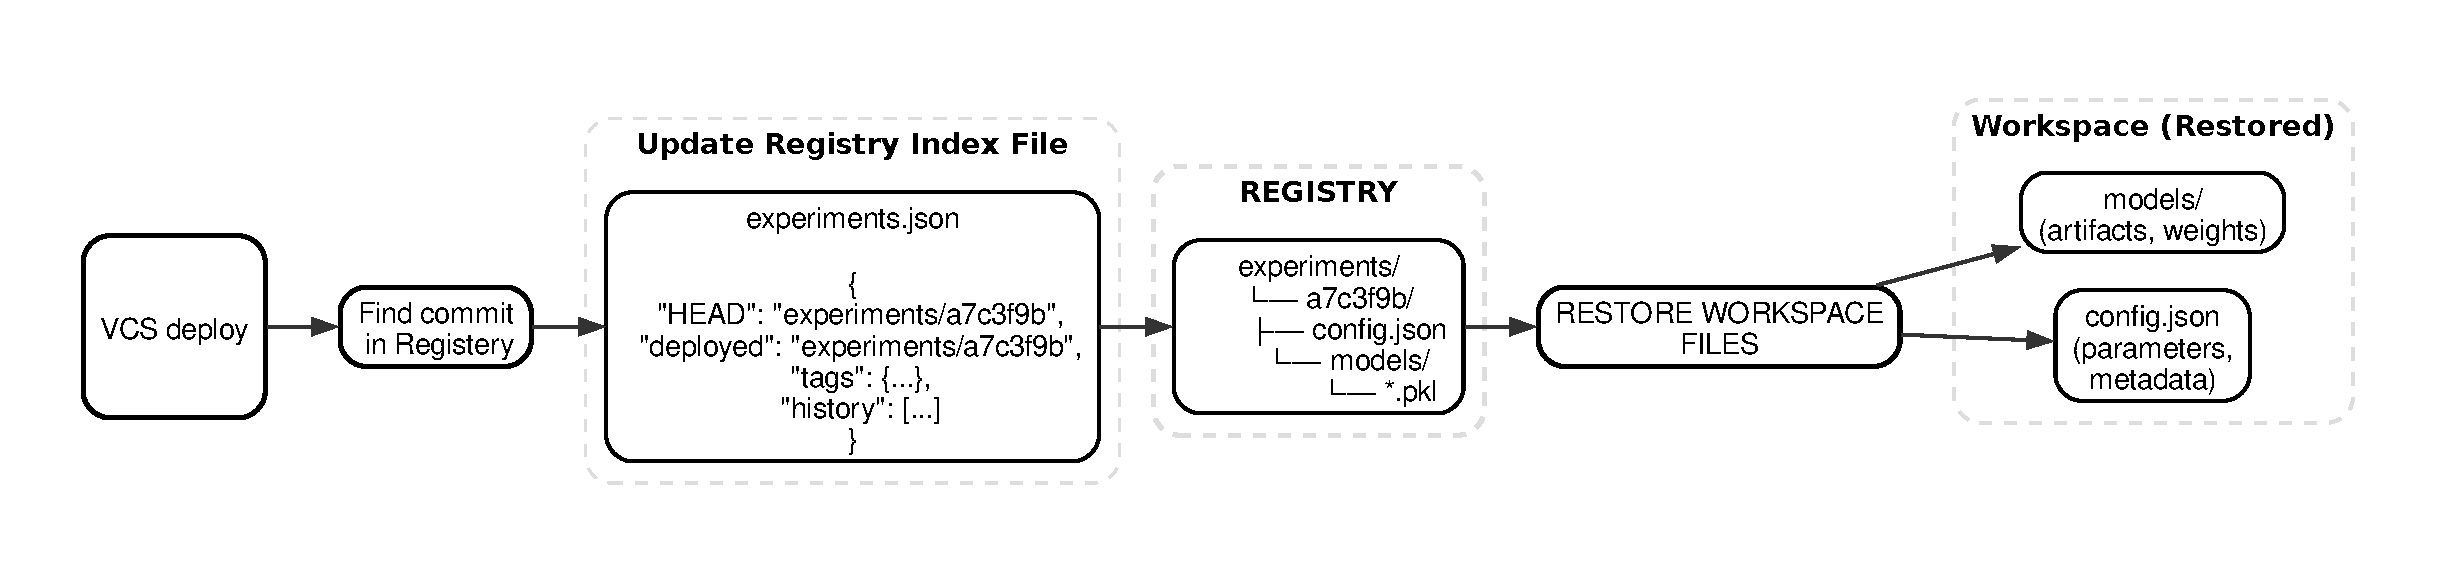
\includegraphics[width=1.2\textwidth]{dots/deployment_deploy.pdf}}
\caption{VCS Deploy Workflow}
\label{fig:vcs_deploy_flow}
\end{figure}

\subsection{Command-Line Interface and CLI Commands}
\noindent The orchestrator and version control features are exposed to the user through command-line interfaces inside \modulepath{deployment.py} and \modulepath{vcs.py}. The supported commands and their behaviors are:

\subsubsection{Orchestrator Commands}
\begin{itemize}[leftmargin=*]
  \item \textbf{prepare}: Prepares the deployment staging area. It copies service modules (e.g. \texttt{server.py}, \texttt{modelservice.py}) and the \texttt{accelera} source library to the \texttt{accelera\_deployment} folder, and generates the serving \texttt{Dockerfile} and \texttt{requirements.txt}.
  \item \textbf{build}: Builds the local Docker container. It invokes local subprocess shell commands (e.g. \texttt{docker build -t <image\_name> .}) with an optional \texttt{--no-cache} flag.
  \item \textbf{run-local}: Starts the local Docker container. It stops and removes any conflicting containers on the port before launching the container using port mappings.
  \item \textbf{local}: Orchestrates the complete local container pipeline by sequentially running the \textbf{prepare}, \textbf{build}, and \textbf{run-local} steps.
  \item \textbf{heroku-login}: Logs the client environment into the Heroku CLI and Heroku Docker registry.
  \item \textbf{heroku-deploy}: Packages and deploys the container to Heroku. It triggers login, pushes the docker image to Heroku's registry, and releases the container for traffic.
  \item \textbf{heroku-push} and \textbf{heroku-release}: Granular command calls that push the container image and release it separately.
  \item \textbf{ec2-deploy}: Deploys to a remote AWS EC2 instance. It establishes an SSH connection, synchronizes files using \texttt{rsync}, compiles/builds the Docker container on the host, runs it, and probes local health targets.
  \item \textbf{ec2-status}, \textbf{ec2-logs}, and \textbf{ec2-stop}: Operational tools to verify container execution, read Uvicorn outputs, and terminate the container on the target EC2 node.
\end{itemize}

\subsubsection{Version Control Commands}
\begin{itemize}[leftmargin=*]
  \item \textbf{init}: Sets up a new model version control workspace by initializing directories and registries.
  \item \textbf{commit}: Snapshots active model parameters and configurations under a message flag (\texttt{-m}).
  \item \textbf{log}: Prints the history log of all model commits.
  \item \textbf{show}: Prints the configuration dictionary details of a target commit.
  \item \textbf{deploy}: Restores a specified commit back into the staging area for subsequent deployment execution.
\end{itemize}

\subsection{Design Constraints}
\noindent The design of the Deployment module is subject to several key constraints:
\begin{itemize}[leftmargin=*]
  \item \textbf{Package Size Optimization}: To minimize container build times and storage footprints, heavy libraries like PyTorch or TensorFlow are excluded from the serving runtime unless explicitly required by the model.
  \item \textbf{Non-Interactive Execution}: Staging and EC2 orchestration must run headlessly in CI/CD pipelines, necessitating automatic Docker installs and automated SSH host key acceptance (\texttt{StrictHostKeyChecking=accept-new}).
  \item \textbf{I/O Isolation}: Process and SSH connection errors are caught as base \texttt{OSError} types to provide descriptive feedback on firewall and network issues without interrupting local execution.
\end{itemize}
